%%%%%%%%%%%%%%%%%%%%%%%%%%%%%%%%%%%%%%%%%%%%%%%%%%
%
%  New template code for TAMU Theses and Dissertations starting Fall 2012.  
%  For more info about this template or the 
%  TAMU LaTeX User's Group, see http://www.howdy.me/.
%
%  Author: Wendy Lynn Turner 
%	 Version 1.0 
%  Last updated 8/5/2012
%
%%%%%%%%%%%%%%%%%%%%%%%%%%%%%%%%%%%%%%%%%%%%%%%%%%%
%%%%%%%%%%%%%%%%%%%%%%%%%%%%%%%%%%%%%%%%%%%%%%%%%%%%%%%%%%%%%%%%%%%%%%
%%                           SECTION IV
%%%%%%%%%%%%%%%%%%%%%%%%%%%%%%%%%%%%%%%%%%%%%%%%%%%%%%%%%%%%%%%%%%%%%

\chapter{\uppercase{Implementation}}

The main goal of Seismic Data Analytics SDK is to develop a scalable and distributed software development tool to enable scalable computation and analytics of seismic volume datasets. This chapter will present the software architecture and the main functionalities of SDK, as well as some utilities we have built for user to deploy their applications on this big data platform.

\section{Architecture}

Seismic Data Analytics SDK is built upon Apache Hadoop and Spark. Figure \ref{sdk_swstack} shows the software stack of a workable seismic data analytics platform. In this diagram, the gray part is the OS layer, the elements with green color stands for the infrastructure layer of this big data platform, and on top of that, SDK layer consists of the components with blue color. At the bottom of the infrastructure layer, there is Hadoop Distributed File System (HDFS) that stores the big seismic data files by utilizing the large number of local disks. The Cassandra as a NoSQL database is also used to store  seismic data, intermediate results and meta data. YARN and Mesos are used for resources management. Apache Spark is the data distribution and parallel execution engine based on the innovative idea of Resilient Distributed DataSets (RDD) concept. MLLib is included in the Spark as the machine learning package to enable machine learning based data analytics algorithms. OpenCV is the widely used image processing package that is used to provide image processing capability. Breeze is the numerical processing package including linear algebra, signal processing, statistics, and other numerical computation and optimizations written in Scala. We have developed the seismic data RDD on top of Spark as the base distributed seismic datasets to enable parallel operations and machine learning algorithms. Geophysicists and data scientists can use  Seismic Data Analytics SDK to develop their own algorithms and leverage the capability of Apache Spark, as well as image processing, numerical computation, and deep learning packages.

\begin{figure}[h]
\centering
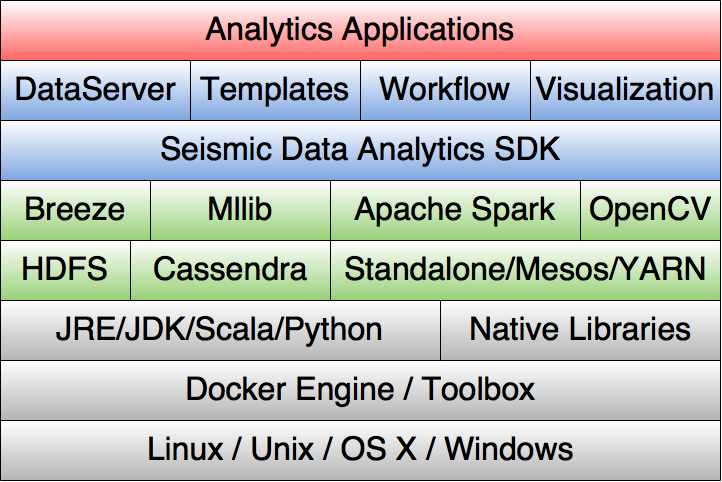
\includegraphics[scale=0.4]{figures/sdk_swstack.png}
\caption{Software Stack of Seismic Data Analytics Platform}
\label{sdk_swstack}
\end{figure}

Figure \ref{sdk_framework} simplifies the development efforts for scalable and distributed computing and analytics of seismic datasets. It is built on top of the Apache Hadoop and Spark. The Hadoop provides a distributed file system(HDFS) and resource management system (YARN and Mesos), while Spark provides a high-level distributed data representation via Resilient Data Sets (RDD) and a data-parallelism execution engine. Seismic Data Analytics SDK provides configurable data distribution fashions for seismic volume data, as well as a configurable parallel execution interface to simplify the parallel programming efforts. Based on the functionality of SDK, we developed two useful utilities, parallel templates and data server, to facilitate SDK for users to easily deploy their applications. Moreover, since Hadoop and Spark provide faults tolerance and task scheduling utilities, the toolkit inherits from them to provide fault tolerance and dynamic task scheduling for better reliability and task management.

The host programming language of Seismic Analytics SDK is Scala (The acronym for Scalable Language), an object-oriented and functional language, which provides great scalability in developing safe and high efficient multi-threaded programs \cite{ScalaOrg}. The most important reason of this is Scala is also the native host language of Apache Spark which means it's the most efficient programming language of this project. Moreover, Scala runs on the JVM which determines it can be freely integrated with Java and Java libraries and tools are also available. Since Scala compiler contains a subset of a Java compiler, users can develop their applications in Java and apply them to Seismic Analytics SDK without putting extra efforts on learning a new programming language.

\begin{figure}[h]
\centering
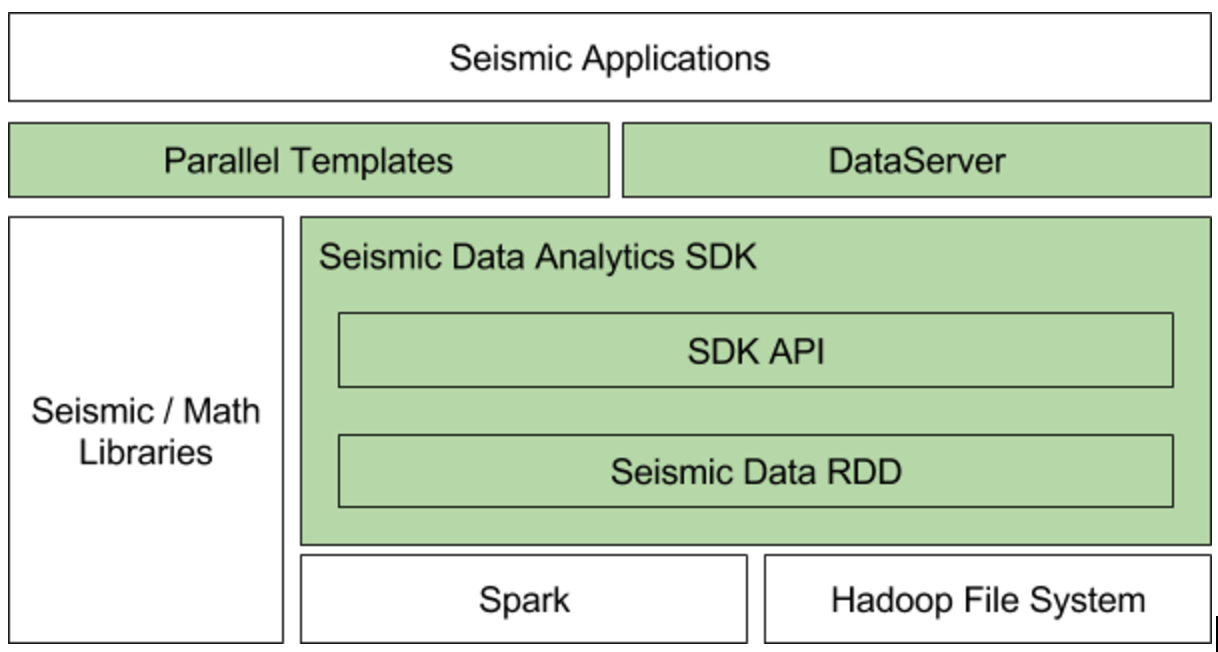
\includegraphics[scale=0.6]{figures/sdk_framework.png}
\caption{Framework of Seismic Data Analytics SDK}
\label{sdk_framework}
\end{figure}


\section{Interfaces and Functionalities}

Figure \ref{sdk_interface} shows the main functionalities of Seismic Data Analytics SDK, including data loading/saving, configurable distribution, data accessing, 3D transpose and user-defined function mapping. It provides a single public class \emph{SeismicVolume}, which integrates all the APIs of SDK. Developers are able to create \emph{SeismicVolume} instances for specified seismic dataset, access data by configurable grain, perform 3D transposing and apply user function to the distributed data instance, and finally save the result to distributed file system through save API. The invalid input data format include 3D binary data and SEG-Y file \cite{SEGDREV21} which is one of the most widely used industrial standard format for seismic data.

\begin{figure}[h]
\centering
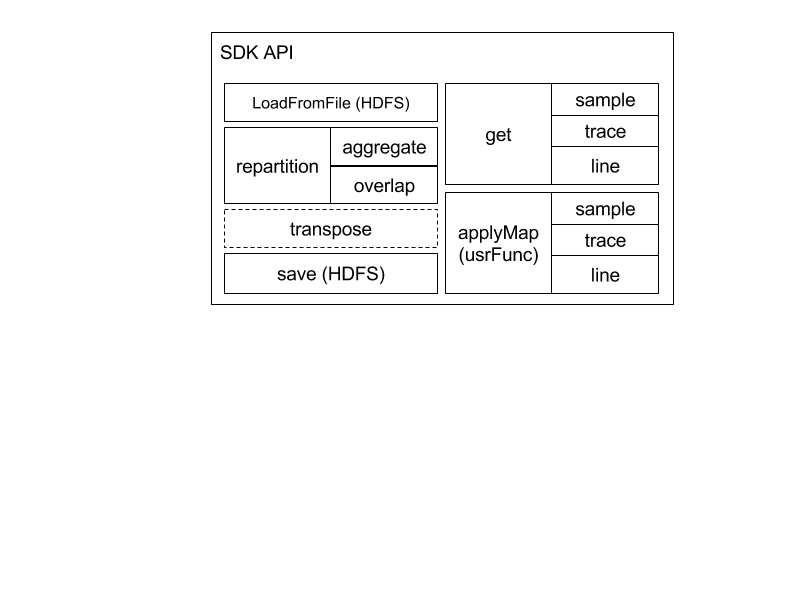
\includegraphics[scale=0.6]{figures/sdk_interface.png}
\caption{Main APIs of Seismic Data Analytics SDK}
\label{sdk_interface}
\end{figure}

\subsection{Seismic Volume Data Loading, Distribution and Saving}

As mentioned in chapter 1, seismic 3D volume data is a collection of estimated property values of the Earth's subsurface, obtained through seismic reflection survey and organized in 3D spacing form. It is widely used in energy companies for geophysics analysis, which could conduct more accurate subsurface exploration and exploit. As shown in Figure \ref{seisdata}, the seismic volume data is defined through 3 different directions in 3D space: inline, crossline and timeline. The industry usually stored the data slice by slice along crossline direction and each slice is a inline section, which is also the default data organization format of Seismic Data Analytics SDK. In this case, each inline slice is a single split of the whole dataset.

\begin{figure}[h]
\centering
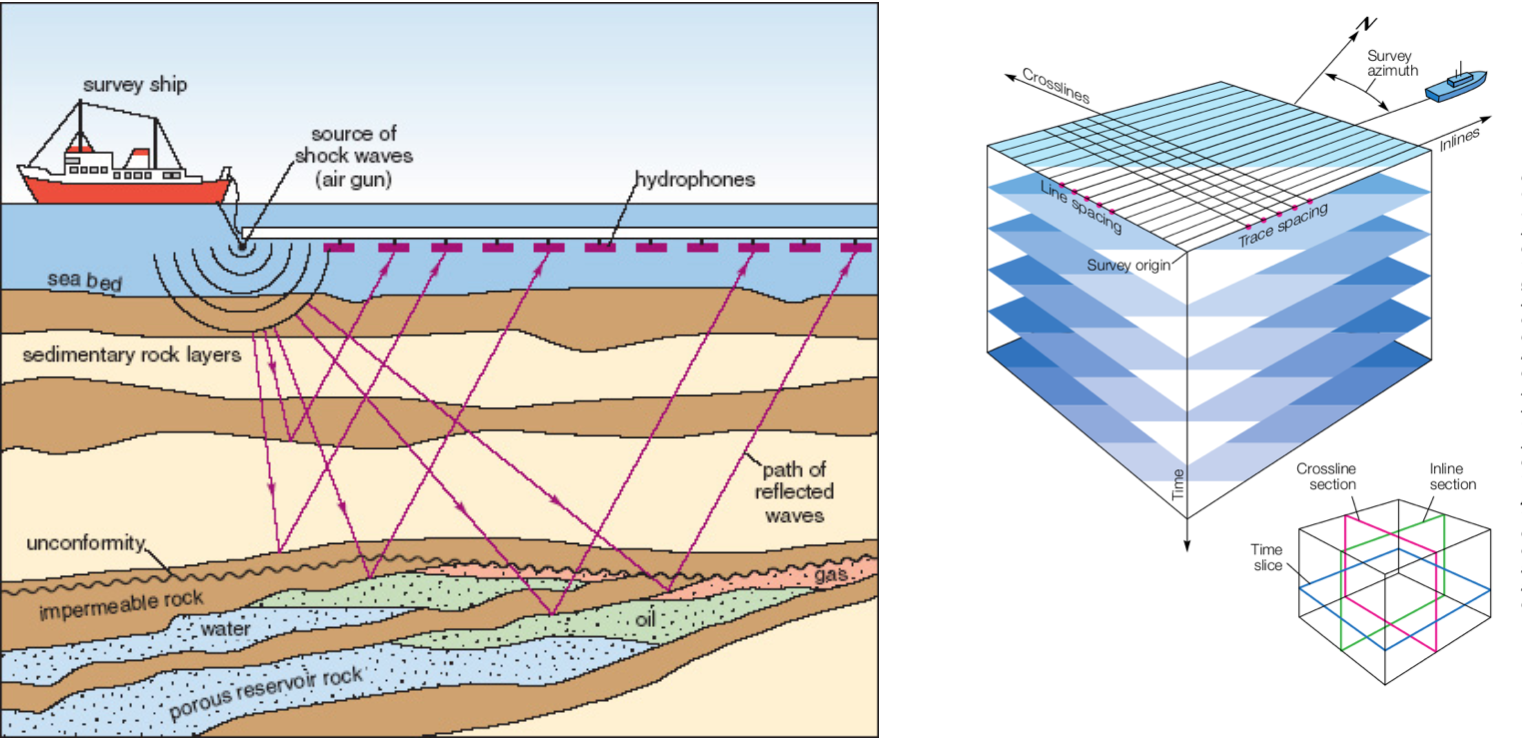
\includegraphics[scale=0.6]{figures/seisdata.png}
\caption{Reflection seismology Survey and Seismic Volume Data \cite{seisaov} \cite{seisinline}}
\label{seisdata}
\end{figure}

The public class \emph{SeismicVolume} provides an API \emph{loadFromFile()} to load seismic data from HDFS and distribute them over Spark RDD according to user?s configurations. This API generates a \emph{SeismicVolume} instance which contains a SeismicRDD with float/byte as internal binary data types. The SeismicRDD is a derived class from Spark RDD class with a variety of distributed fashions of seismic volume data. In addition, it also provides some optional parameters for advanced users who have already familiar with distributed system to specify the advanced data distribution fashions. 

Figure \ref{datadist} shows the flow of distributing an seismic volume file through the Hadoop filesystem and Spark RDD. It assumes the file has already been uploaded to Hadoop file system, which is able to support the distributed IO accessing for Spark to load data in parallel. After user get the  \emph{SeismicVolume} instance of a specified file,  all Spark RDD operations can be applied to the inside SeismicRDD object. Utilizing the RDD methods provided by Spark, developer could perform various of data operations and calculations on the dataset in parallel. By default, SDK distributes the volume in inline format slice by slice, which means each partition contains one single inline slice. The distribution direction could also be configured to crossline/timeline by given parameters in other APIs, this function will be present in the following Volume Data 3D Transposing section. User could configure the slices count of each distribution to manage the data distribution grain, thus to efficiently tuning the performance of applications.

\begin{figure}[h]
\centering
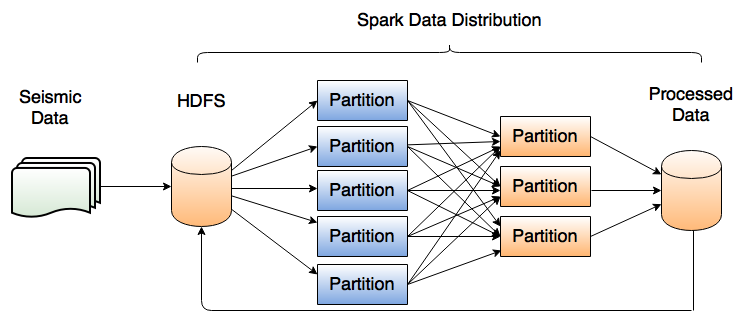
\includegraphics[scale=0.6]{figures/datadist.png}
\caption{Seismic Volume Data Distribution Flow}
\label{datadist}
\end{figure}

\emph{SeismicVolume} class also provides \emph{save()} API to allow user to store the data of SeismicRDD back to the HDFS. Although this operation is not recommended since it could introduce performance issues caused by data shuffling, it is still necessary when user need to backup the runtime data or apply the runtime data to traditional sequential workflows.


\subsection{Volume Data Accessing}

Seismic Data Analytics SDK allows users to to access any slice/trace/sample data in any direction of the volume through \emph{SeismicVolume} APIs \emph{getLine(direction:Int, idx:Int):Array[T]}, \emph{getTrace(dir:Int, i:Int, j:Int):Array[T]} and \emph{getSample(i:Int, j:Int, k:Int):T}. 
For the convenience of addressing the data organization, we defined the three dimension of seismic volume as I (Dimension of inline slices), J (Dimension of crossline slices) and K (Dimension of timeline slices), as shown in Figure \ref{VolumeDim} and Figure \ref{VolumeTrans}. Users can specify any one of I, J and K directions to access data for visualization or computation purpose. Since Spark does not provide arbitrary data access, the APIs used IndexedRDD, a more efficient key-value management than native Spark API \cite{IndexedRDD}, to implement and speedup queries of slice/trace/sample data from any distributions to the master node.

\begin{figure}[h]
\centering
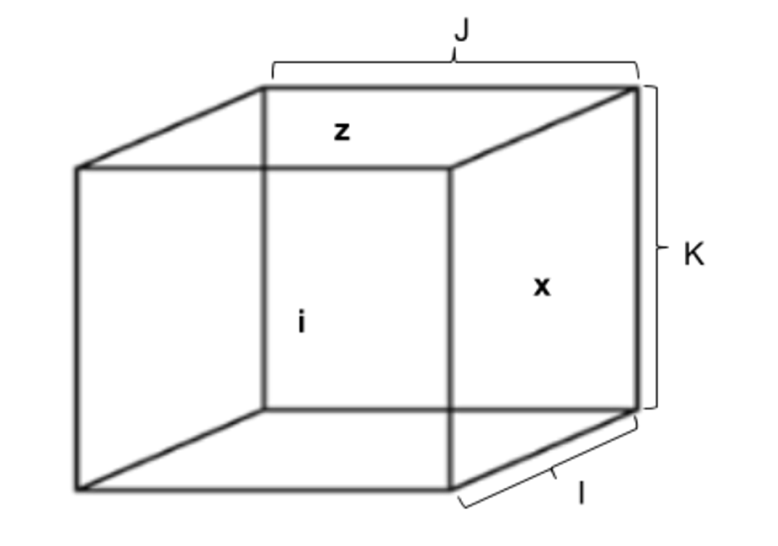
\includegraphics[scale=0.6]{figures/VolumeDim.png}
\caption{Seismic Volume Data Dimensions}
\label{VolumeDim}
\end{figure}


\subsection{Volume Data 3D Transposing}

Since the volume data could only be stored in file following one specific direction(I, J or K), developer could not access slices of the other two directions directly. In traditional solutions, if user needs data in other directions, organized as cross-line slice or time-line slice, the data fetching program must perform lots of seek operations between different file offsets to collect the data of a single cross-line or time-line slice. This tedious procedure will dramatically slow down the whole software performance. To resolve this problem and to achieve reasonable performance, SDK handles the transposing of the 3D volume data inside the \emph{SeismicVolume} APIs and caches all three directions format SeismicRDD in \emph{SeismicVolume}.

To explain the implementation clearly, we denote the seismic volume data as shown in Figure \ref{VolumeDim}, in which i means I slice, x means J slice and z stands for K slice. The data is stored in iSlices format by default. To resolve the transposing problem in each distribution evenly, we split the volume to I of iSlices and distribute them over SeismicRDD. Each iSlice is a 2D matrix. As shown in Figure \ref{VolumeTrans}, each iSlice matrix consists of J of iTraces which have the length of K. An iSlice matrix could be iterated iTrace by iTrace. Since in 3D spacing, each iTrace is also the trace of xSlice, for example, the iTraces(0) is the xTrace of the 0th xSlice, the iTraces(1) is the xTrace of 1st xSlice, etc. Thus, we implement a map function to index all iTraces of the volume. The new index is combined by index of iTrace and index of iSlice. After indexing the map, we got a volume RDD with new (iTraceIndex)(iSliceIndex) index as the key, trace data as the value. As shown in Figure \ref{VolumeTrans}, to get a xSlice, we need group all the traces with the same iTraceIndex by utilizing the \emph{group} operations of Spark RDD. After grouping, the xSlices data collection is generated in the new SeismicRDD distribution map. To organize them as a xSlices volume, all we need to do is sorting them by iTraceIndex. So far, the data in requested direction has already been stored in the \emph{SeismicVolume} instance, therefore user could access and manipulate seismic data in any direction by specifying the direction parameter of related \emph{SeismicVolume} APIs.

\begin{figure}[h]
\centering
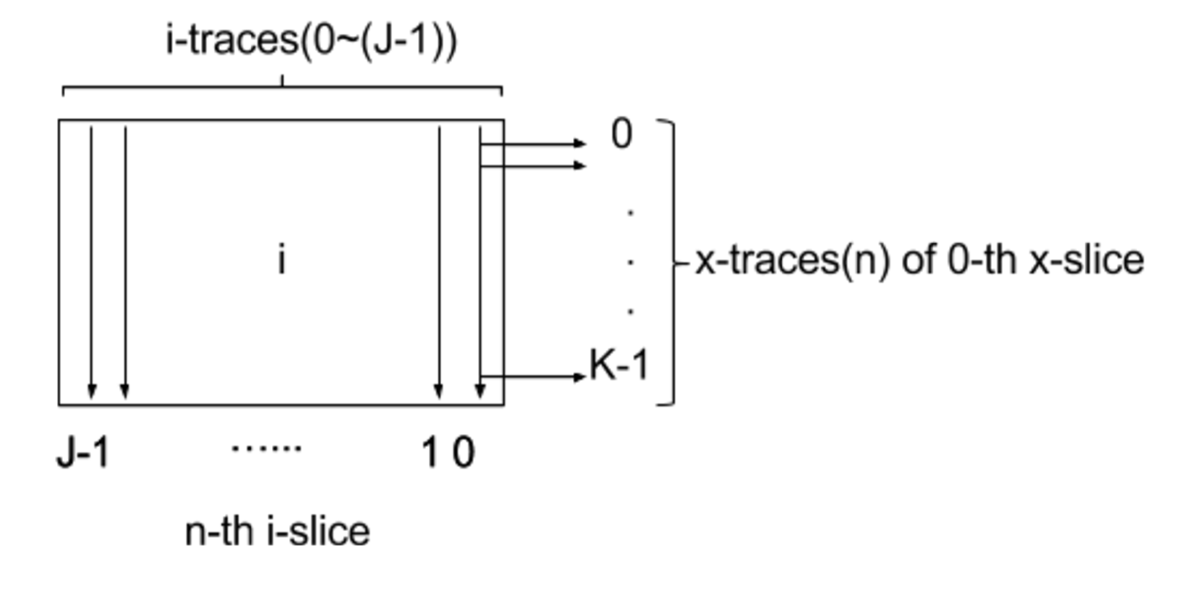
\includegraphics[scale=0.6]{figures/VolumeTrans.png}
\caption{The Indexing for Resolving 3D Transposing Problem}
\label{VolumeTrans}
\end{figure}


\subsection{Aggregation and Overlapping}

By default, as shown in Figure \ref{DefDist}, SDK distributes the volume in one specific direction slice by slice. In this case, each slice is a single split of the whole dataset. However, it will cause performance problems for some applications if we only support one distribution. For an instance, the transposing solution as mentioned in previous section needs to do lots of data exchanges between different data splits for the \emph{group} operation to shuffle the dataset to expected arrangement. Since data shuffle in Spark RDD relies on lots of physical storage access and network transmissions in each worker node, it will become the bottleneck of the transposing performance if the number of partitions is too big. Obviously, to speedup the transposing operation, user need to reduce the number of partitions thus to reduce the data communications between worker nodes. Therefore, user need a way to configure the data split size and partition number so they can tuning the performance of their programs.

Developers can change the distribution layout to the aggregated and overlapped fashions as shown in Figure \ref{Aggregation} and Figure \ref{Overlap} by utilizing the \emph{SeismicVolume} API :

 \emph{repartition(planesPerMap:Int,overlapPlanes:Int):SeismicVolume[T]}.

\begin{figure}[h]
\centering
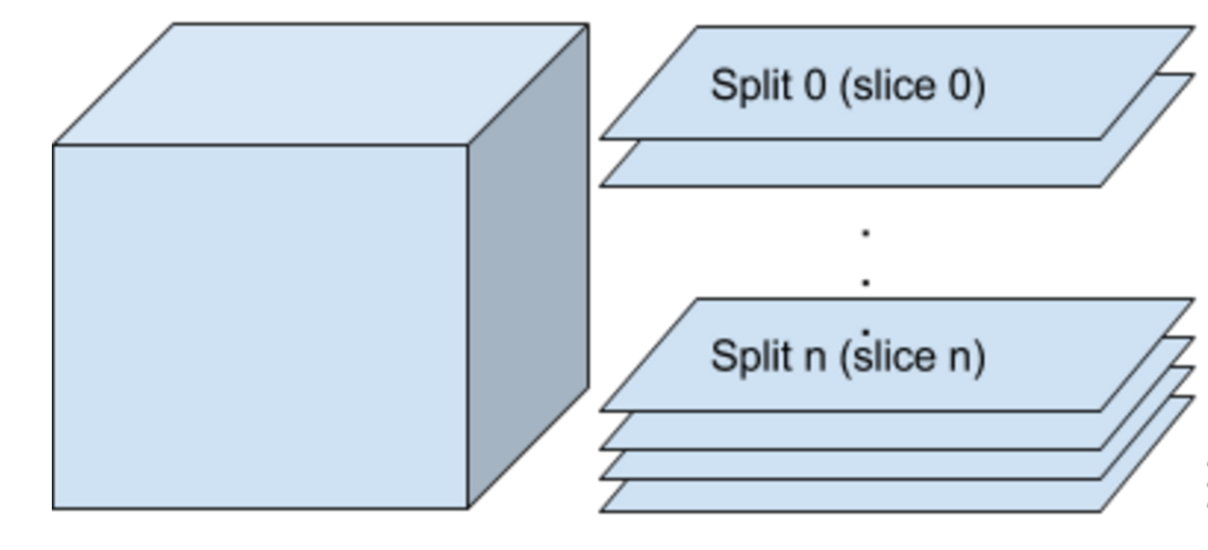
\includegraphics[scale=0.6]{figures/DefDist.png}
\caption{Default Distribution Fashion of Volume, planesPerMap=1, overlap=0}
\label{DefDist}
\end{figure}

As shown in Figure \ref{Aggregation}, aggregated data distribution could be achieved by utilizing the RDD group operations we mentioned in Volume Data 3D transposing section. The solution of this problem is to re-indexing all the slices in parallel through RDD map function by arranging an unique key to multiple data splits, then use RDD \emph{groupByKey()} API to repartition the dataset. An aggregated dataset could have multiple slices in a single data split.

\begin{figure}[h]
\centering
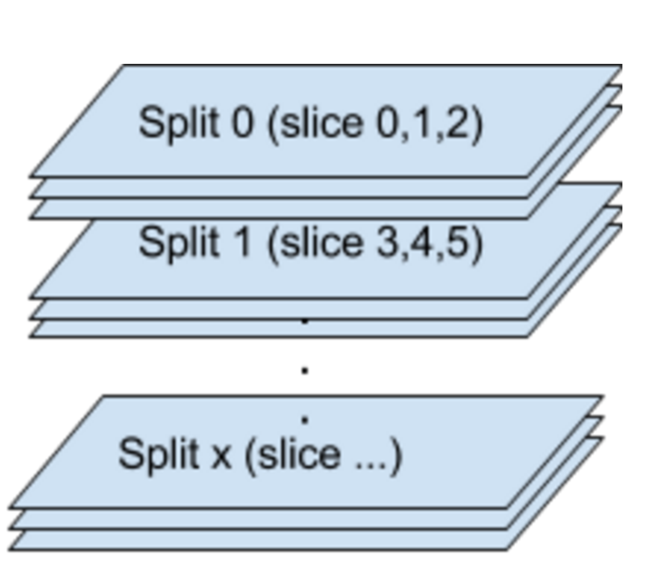
\includegraphics[scale=0.6]{figures/Aggregation.png}
\caption{Aggregated Distribution of Volume, planesPerMap=3, overlap=0}
\label{Aggregation}
\end{figure}

This method not only lets user change the size of distributed splits, more powerfully, it allows developer to set the overlapped data areas between splits and to access the overlapped parts in each split. Practically, some applications may have strong data dependences in their logic which is very hard to parallelize the solutions. For example, the stencil computation needs lots of data communications between neighbor units in each step, which is impossible to run it in parallel with other MapReduce frameworks. 

To resolve this problem, \emph{repartition()} API generates the head and tail boundaries RDD on top of the aggregated SeismicRDD and indexing them according to the related partition numbers. Finally, the boundaries are appended to each related data split through RDD \emph{zip()} API to generate a new \emph{SeismicVolume} instance which contains overlapped SeismicRDD. 

\begin{figure}[h]
\centering
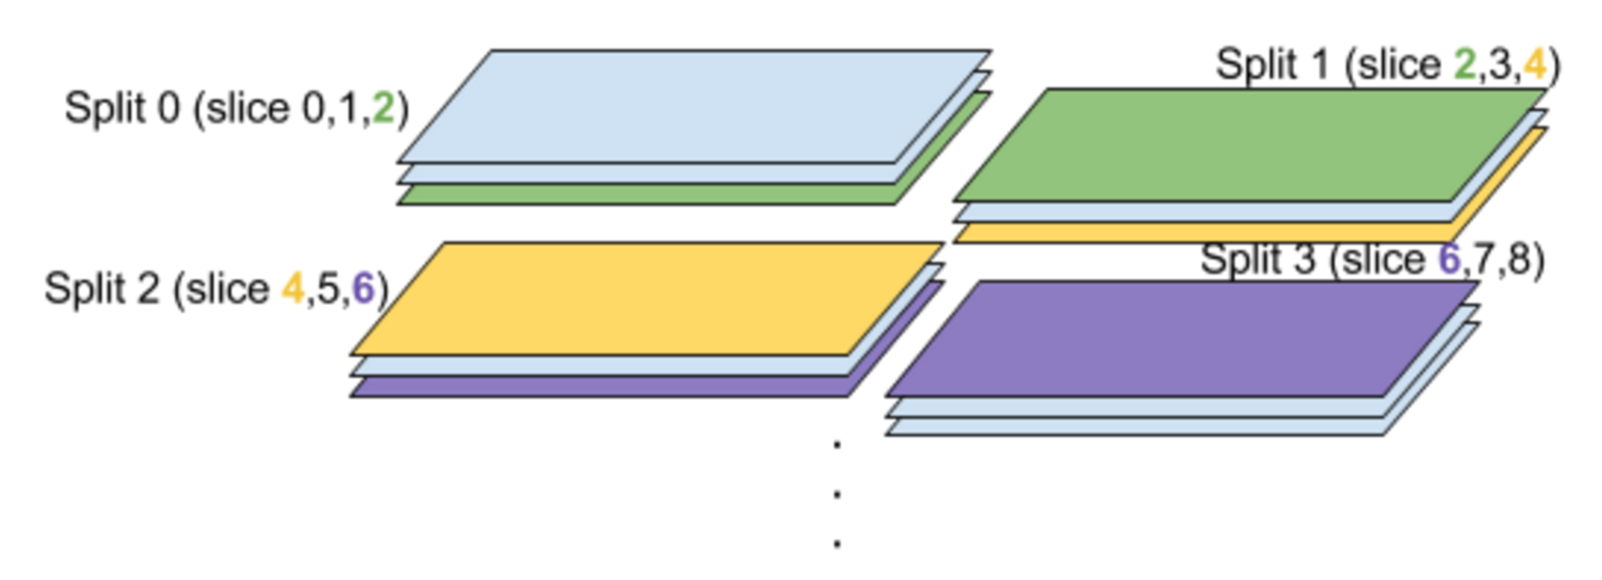
\includegraphics[scale=0.5]{figures/Overlap.png}
\caption{Overlapped distribution of Volume, planesPerMap=1, overlap=1}
\label{Overlap}
\end{figure}

Therefore, this method is not only capable of tuning the performance of distributed tasks, but also simplifies the stencil-style computation requiring neighbor communication, which is not easy to parallelize in MapReduce programming mode. We have developed a more complicated 3D stencil use case with 3D spacing overlapping which will be presented in detail in following Experiments chapter. It could be used for resolving seismic 3D attributes computation problem.


\subsection{User Defined Function Mapping}

As mentioned in Introduction chapter, one of the project objective is to provide an easy-to-use solution for geophysicists or data scientists to apply their programs on big data platform without concerning the parallelism and code reconstruction. To achieve this, \emph{SeismicVolume} provides \emph{applyMap()} API to allow developer to apply user-defined functions on any direction of the SeismicRDD in parallel. 

The prototype of this API is \emph{applyMap(direction:Int, f:(T-U))}. The first parameter \emph{direction} indicates the direction that user would like to apply the function on. The other parameter \emph{f:(T-U)} is a standard spark RDD key-value pairs operation callback function, which feeds the function distributed volume data with key-value forms in parallel. The data length in each key-value function depends on the specified distribution parameters of the target \emph{SeismicVolume}.  User could apply any operation or computations on the given input data, and an output key-value pairs is required for the return value. This callback function will be executed along with the related data distribution in parallel. After execution, it will generate a new \emph{SeismicVolume} object containing the processed and distributed dataset output by user-defined function.  Figure \ref{code_apply} shows the example code for users to apply their function.

\begin{figure}[h]
\centering
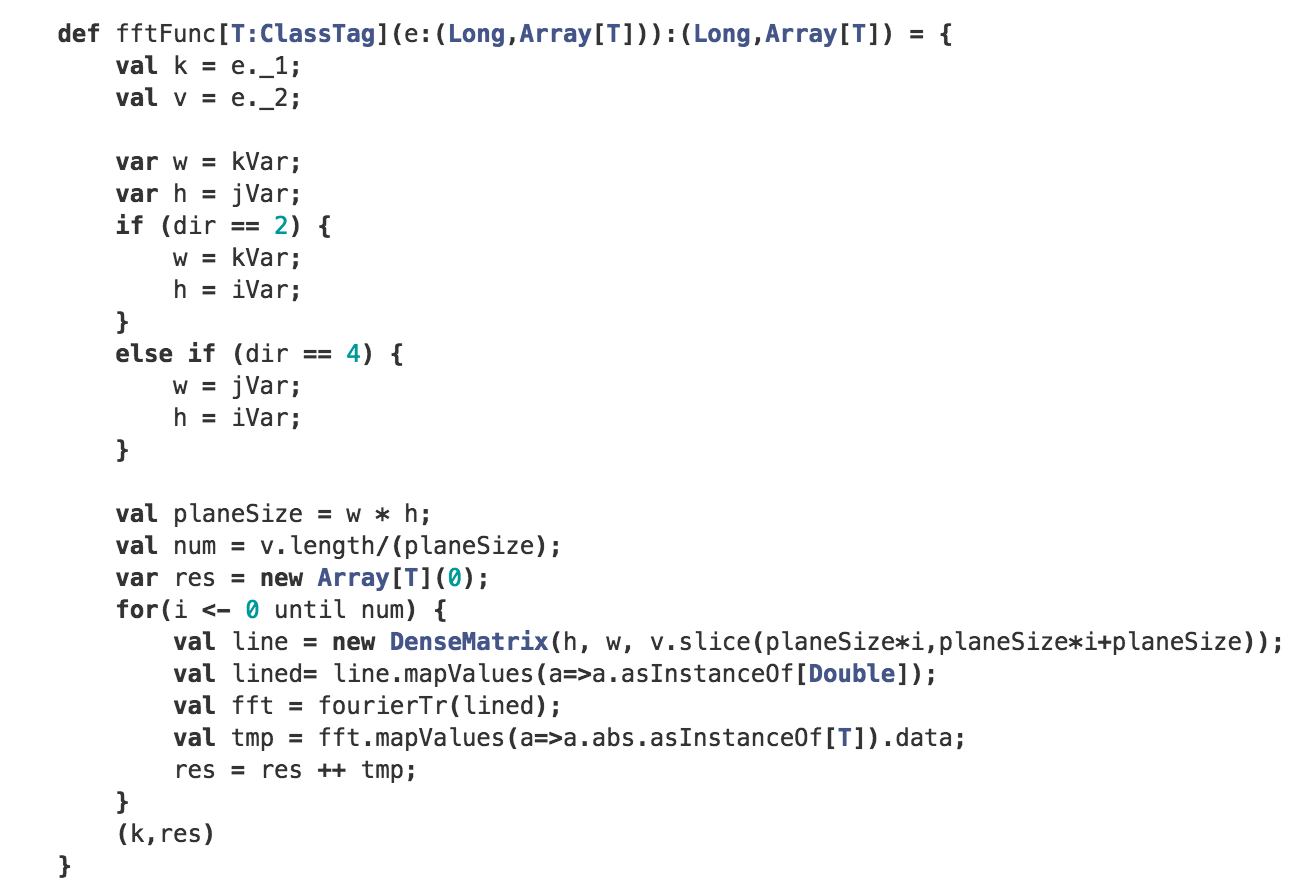
\includegraphics[scale=0.6]{figures/code_apply.png}
\caption{Sample Code for Applying User-defined function in Parallel}
\label{code_apply}
\end{figure}


\section{Application Utilities}

Data distribution plays an important role in distributed parallel programs to achieve scalable performance. However, most scientists and researchers in petroleum industry do not have enough big data background knowledge to support them to convert their work to Spark applications. To overcome the usability barriers, we developed some utilities on top of Seismic Data Analytics SDK to simplify the way for deploying general sequential applications on Spark-Hadoop platform, which include several parallel templates for user-defined procedure, a general purpose data server for remote data access, as well as the web interfaces for remote data visualization and user-defined workflow. With these tools, developers could facilitate their works with big data platform in minimal efforts without concerning all the parallelism details.

\subsection{Parallel Templates}

Based on Seismic Data Analytics SDK APIs, we developed several parallel templates to make SDK be easily used by domain algorithm designer other than computer scientists.These templates defines the data distributions and parallel computation so that users can simply select the right templates for their algorithms without handling the data distribution and parallelism details. Three templates currently include: Trace, Line and Sub-volume. Each template can handle one or more volumes, and will output one or more volumes. Trace template is simple, in which the input is a 2D array (dimension 1 for number of volumes and dimension 2 for 1D trace data), and output is also a 2D array. Line template defines a 3D array as input and a 3D array as output respectively (dimension 1 for number of volumes and dimension 2 for 2D slice data, line is the petroleum terminology). Sub-volume template is a powerful solution to handle data 3D data distribution with overlaps, in which both input and output are 4D array (dimension 1 for number of volumes and dimension 2 for 3D overlapped sub-volume data). The Sub-volume template outputs data without any overlapping. Users can specify parameters about how to distribute data as well as the overlapped areas. 

Figure \ref{code_tmpl_line} shows an example of the Line Template and Figure \ref{code_tmpl_subv} shows the example of Sub-volume Template. Both of them are straight forward and require very few knowledge about parallel computing. The only thing user should be aware of is the distribution grain of input/output data, which is specified in the distribution parameter when user creates the template instance. As shown in Figure \ref{code_run_subv}, it demonstrates the execution of an Sub-volume Template instance, in which the distributed input sub-volume size in dimension I and J (for each parallel \emph{proc()} callback function) is set to 26 x 21(The sub-volume size in dimension K is always the complete length of iTrace/xTrace, which is the minimal unit for seismic computation), and the overlapping size is 4 in both I and J direction (Each data split extends to 30 x 25 in I x J).

\begin{figure}[h]
\centering
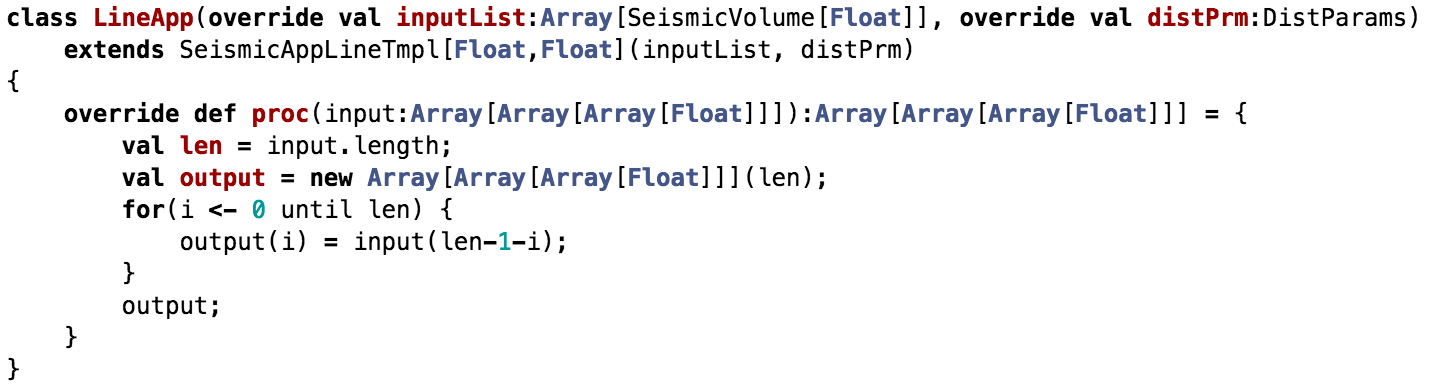
\includegraphics[scale=0.6]{figures/code_tmpl_line.png}
\caption{Sample Code of Line Parallel Template}
\label{code_tmpl_line}
\end{figure}

\begin{figure}[h]
\centering
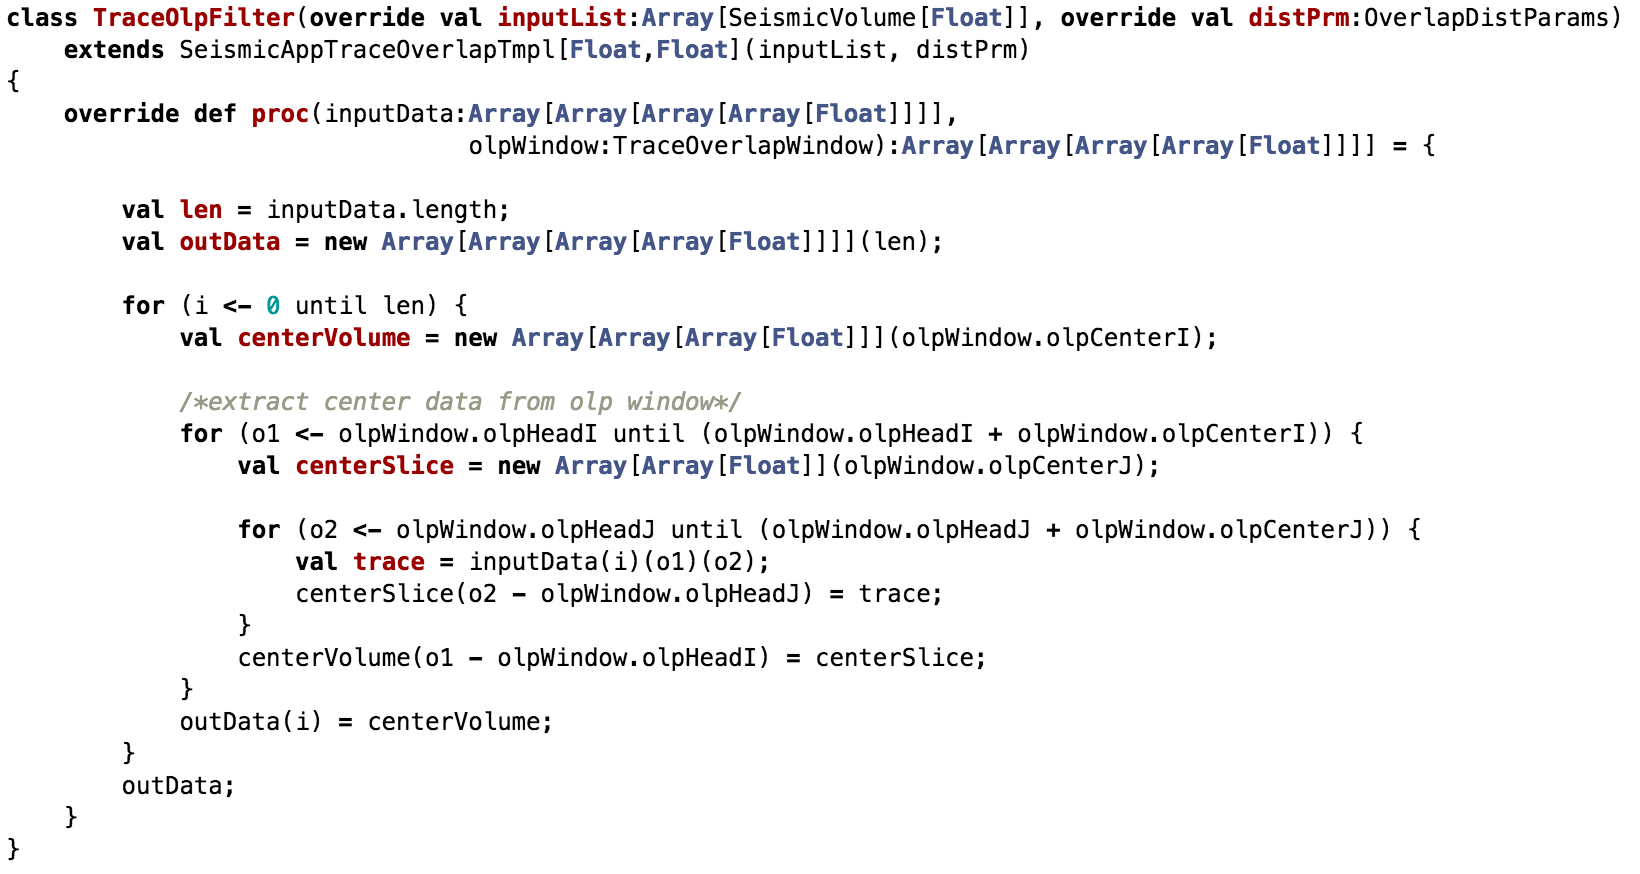
\includegraphics[scale=0.5]{figures/code_tmpl_subv.png}
\caption{Sample Code of Sub-volume Parallel Template}
\label{code_tmpl_subv}
\end{figure}

\begin{figure}[h]
\centering
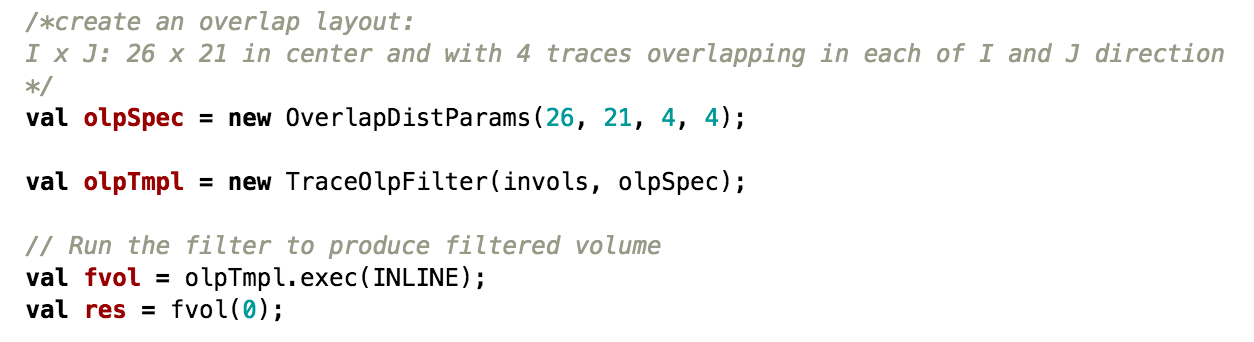
\includegraphics[scale=0.6]{figures/code_run_subv.png}
\caption{Sample Code of Executing Sub-volume Parallel Template}
\label{code_run_subv}
\end{figure}


\subsection{Data Server and Remote Web Visualization}

In petroleum industry, an important application scenario is data visualization, which allows user to browse and analyze seismology features of seismic data in 3D spacing. With visualization tools, computer renders the seismic data to 3D graphic views and allows user to browse and manipulate the graph along any direction, which inspired the geophysicists and data scientists to develop various of useful models. However,traditional visualization tools in industry are only capable of handling small datasets, or render only few segments of the big datasets at a time. The performance of  big dataset visualization has long been the critical bottleneck of regular workflow of industry.

To resolve this problem, we developed a web-based remote data visualization service which is able to load and render the seismic data for 3D visualization in real-time. Figure \ref{visualization_framework} shows the framework of this service. 

\begin{figure}[h]
\centering
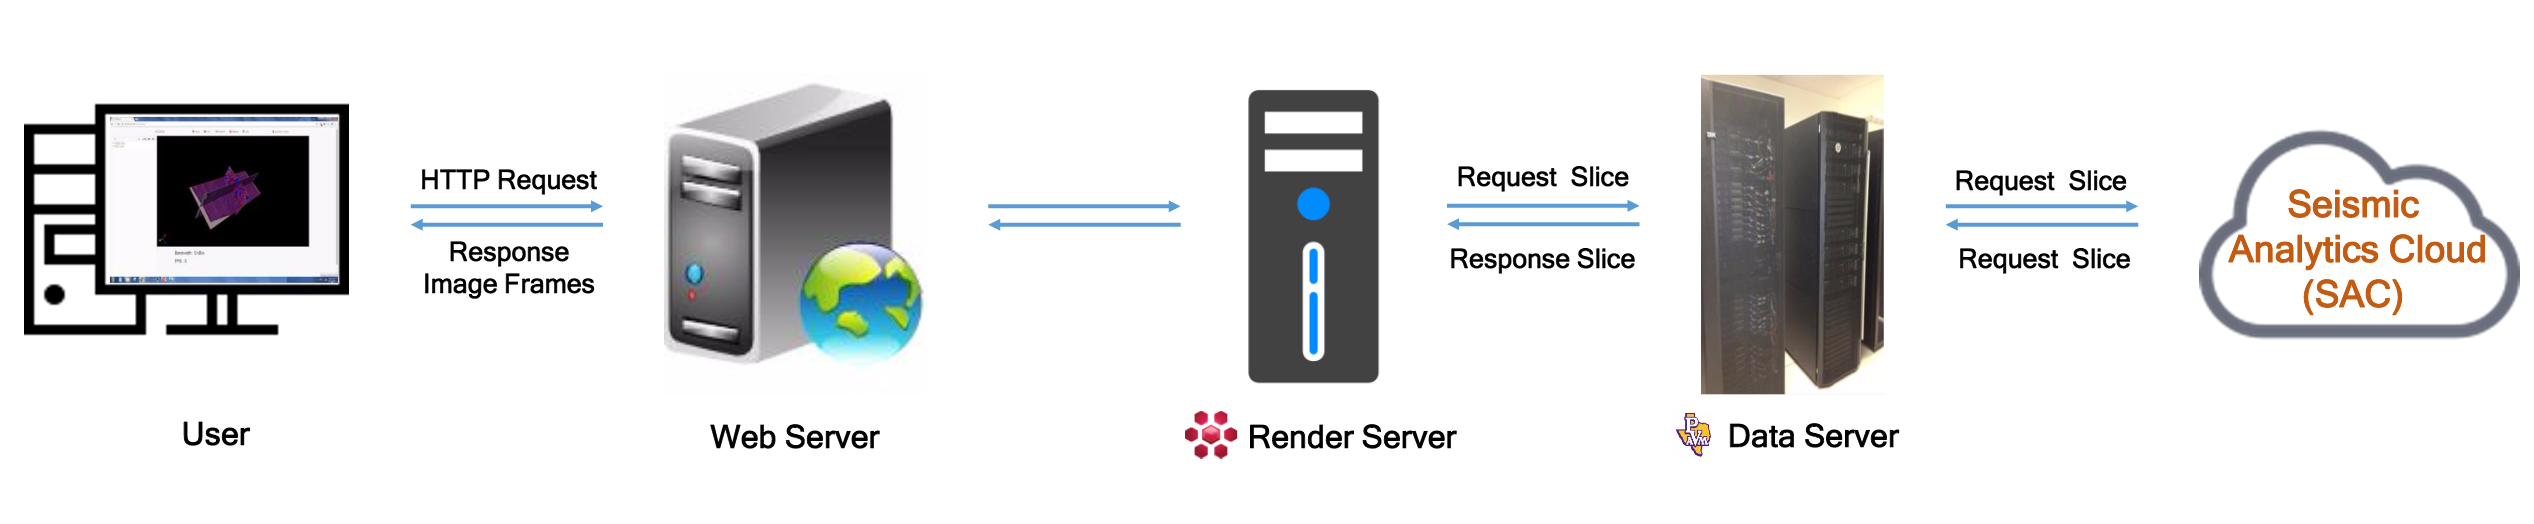
\includegraphics[scale=0.3]{figures/visualization_framework.png}
\caption{The Framework of Remote Web Visualization Service}
\label{visualization_framework}
\end{figure}

This solution is developed on top of Seismic Data Analytics SDK APIs and FEI Digital Rock Visualization Packages. We design and implement the DataServer service on top of Seismic Data Analytics SDK, which could load big seismic datasets from HDFS, transpose and store them to SeismicRDD in backends then feed the requested data in any direction to FEI visualization service in real-time. The FEI Digital Rock Visualization package is developed by FEI, the company which has been focus on featuring Digital Rock technology and solutions many years \cite{FEICompany}. 

Finally, the output rendered data view is presented through web interface and allows user to browse and manipulate in any direction. With this solution, user do not need to install complicated visualization tools and packages since the platform handles everything on server-side. More importantly, the performance of rendering big seismic data is improved and scalable after facilitated by Seismic Data Analytics SDK. Figure \ref{visualization} show s the web interface of this solution.

\begin{figure}[h]
\centering
\includegraphics[scale=0.3]{figures/visualization.png}
\caption{Visualization Web Interface}
\label{visualization}
\end{figure}


\subsection{Web-based Workflow Platform}

Another service we developed is a web-based workflow platform, which provides a friendly web interface to make cloud platform easy to use without programming, with which users could create workflow with drag and drop, could run the created workflow and check the results through visualization model. The Workflow Web Service is implemented on an open source project Clowdflows \cite{Clowdflows}, which provides a Django based framework to develop a customized widget and to manage widgets conveniently. As a free and open source web application framework written in Python, Django follows the Model, View and Controller (MVC) architectural pattern, so it is suitable for interact with both cloud service and web client.

The client side view of workflow is shown as Figure \ref{workflow}. Users could select widgets and specify seismic data files as input to construct and customize their workflows. Each widget in the workflow view is an independent application component which could be implemented on top of Seismic Data Analytics SDK. A widget acquires at least one port as input or output thus multiple widgets are able to be combined to a workflow by multiple pipelines which connect the ports of all widgets. Each pipeline in the workflow view indicates a data communication, which transports data between widgets and drives the execution of whole workflow. The workflow framework implemented by Python code includes Django views (GUI), Django models (widgets data management) and topological sorting algorithm (connections check).  The data files are stored in HDFS of the cloud platform and could be browsed and selected from the navigation trees on the editor page.

\begin{figure}[h]
\centering
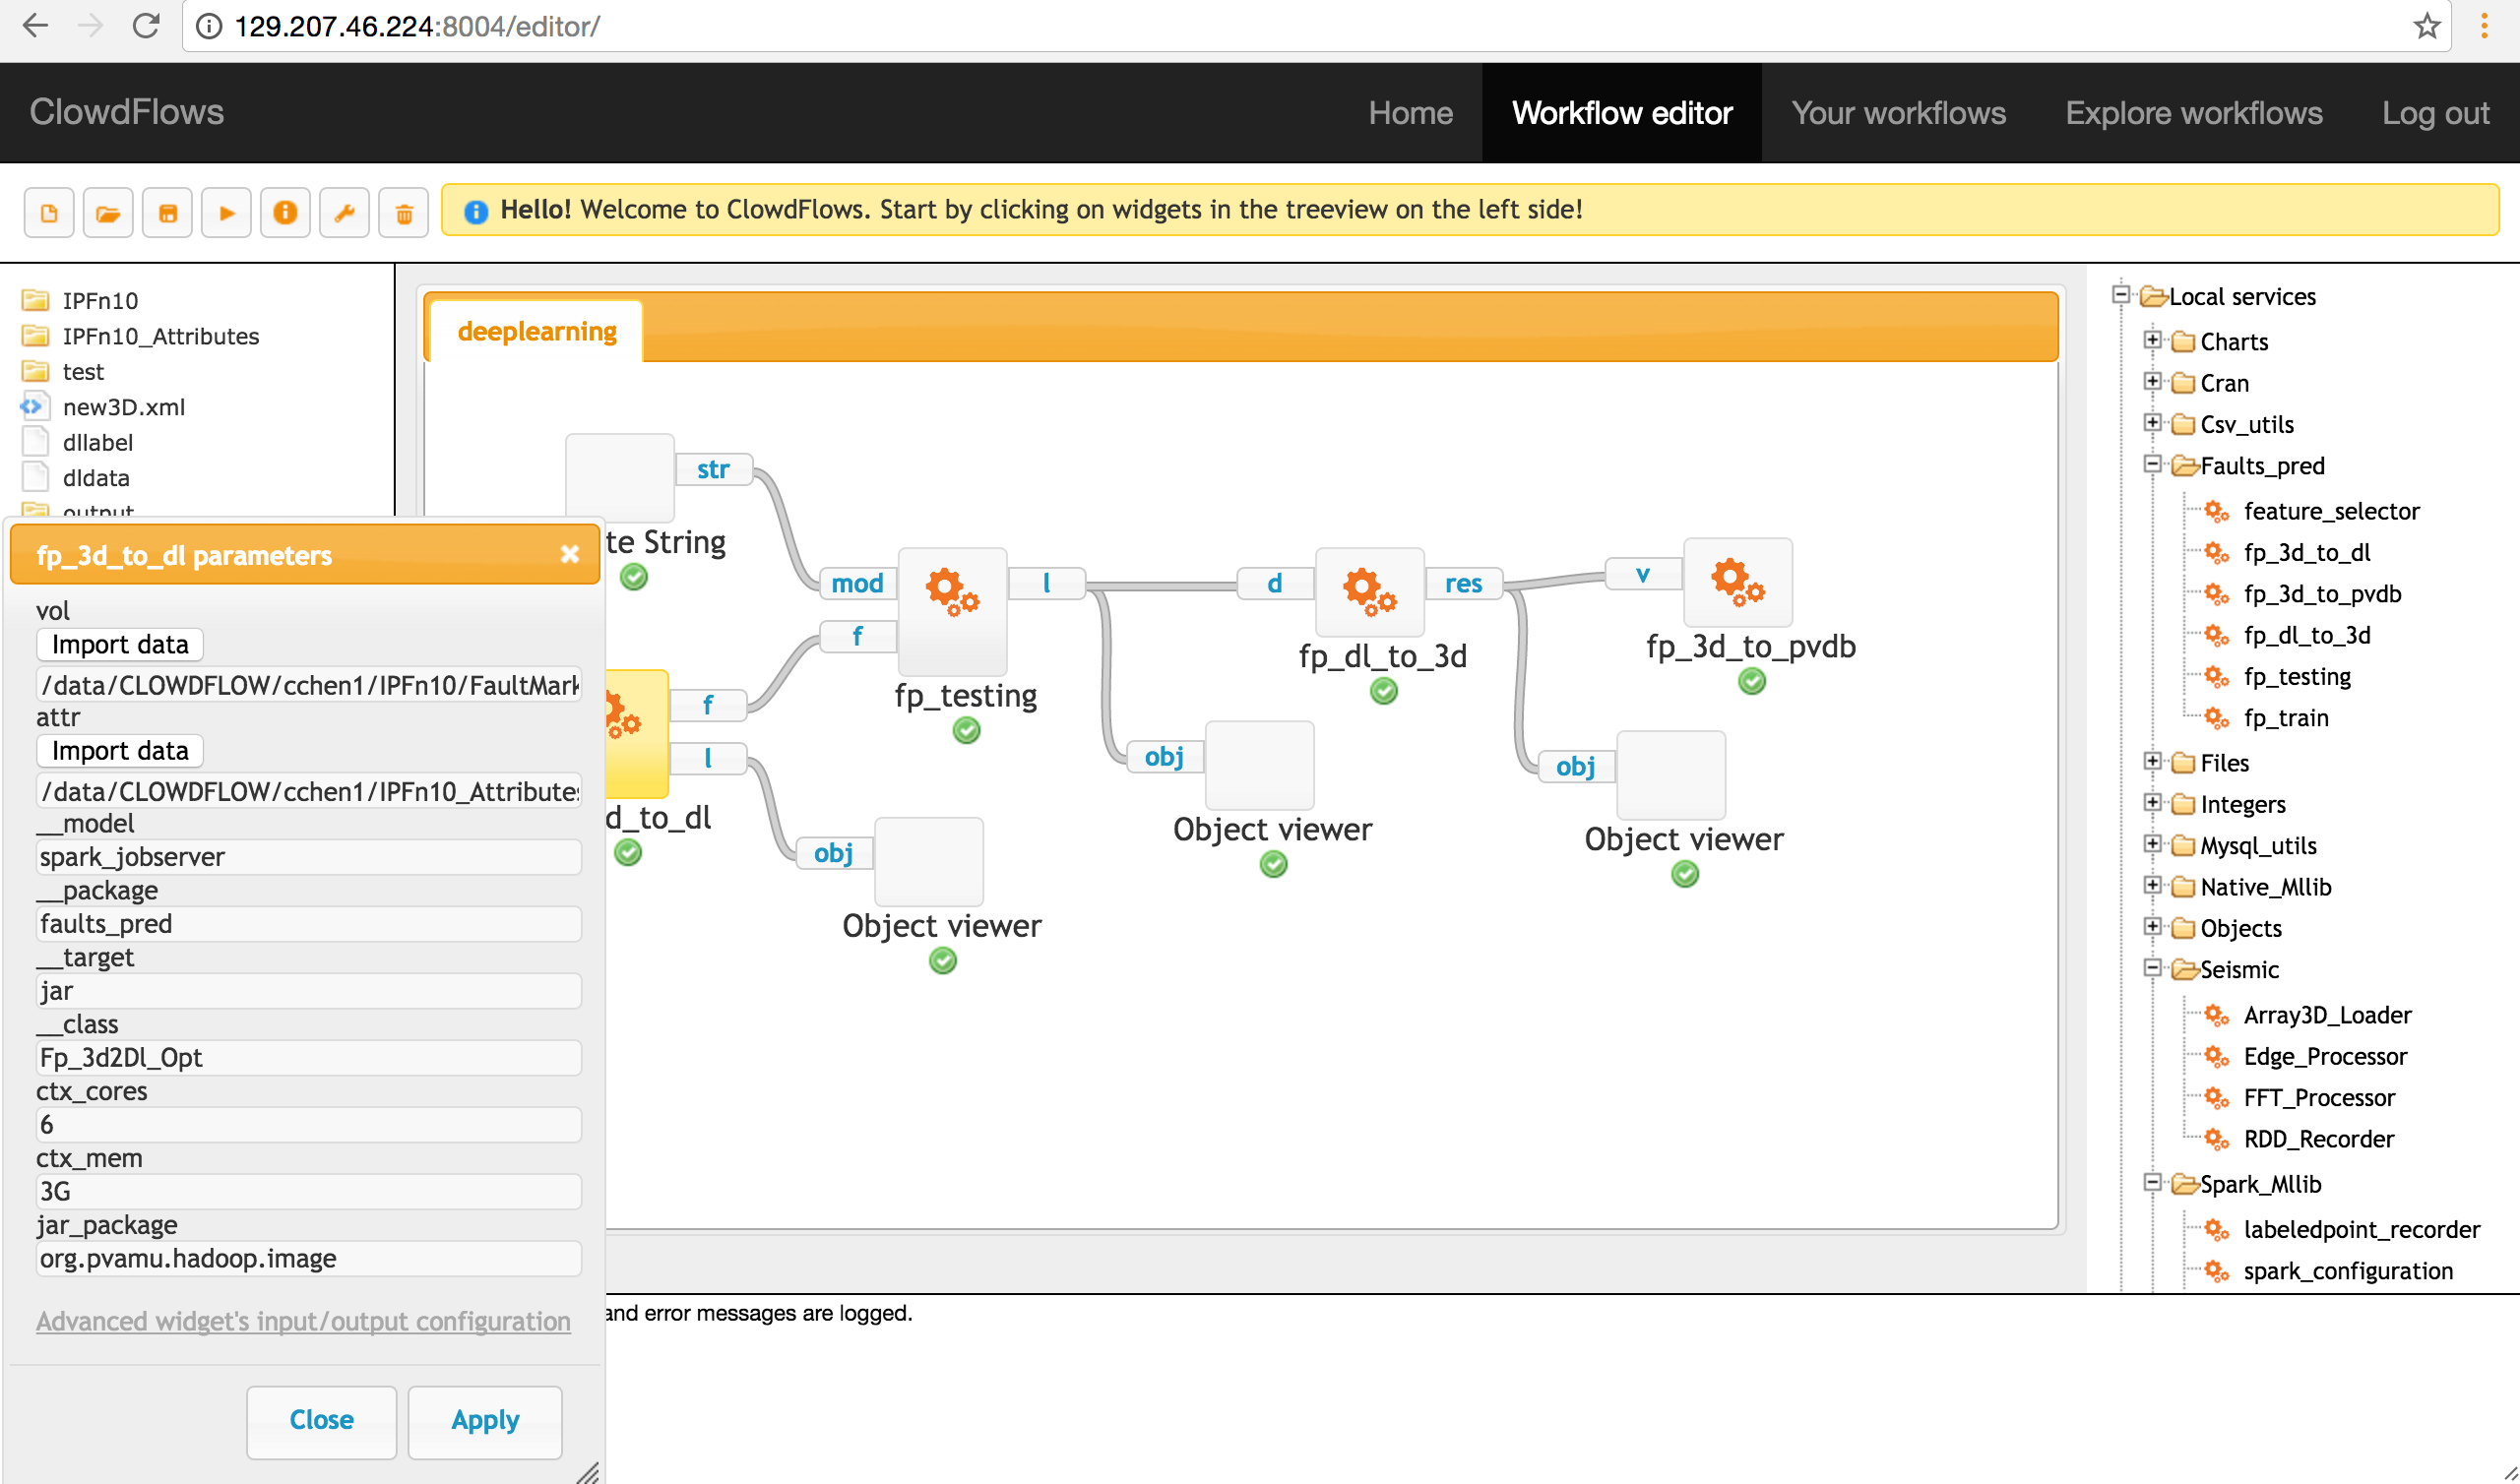
\includegraphics[scale=0.3]{figures/workflow.png}
\caption{Workflow Web Interface}
\label{workflow}
\end{figure}

